%        File: Modeling_the_Formation_of_Rain.tex

\documentclass[twocolumn,a4paper,10pt]{article}
\usepackage{times}
\usepackage{fixltx2e}
\usepackage{amsmath}
\usepackage{amssymb}
\usepackage{graphicx}
\usepackage{float}
\usepackage[usenames,dvipsnames]{color}
\usepackage{subfig}
\usepackage{wrapfig}
\usepackage{gensymb}
\usepackage{array}
\usepackage{listings}
\usepackage{titling}
% Hyperref must be last
\usepackage[backref,colorlinks,linkcolor=blue]{hyperref}

\newcommand{\TODO}{{\huge\emph{\color{red}!}}}

\title{Modeling the Formation of Rain using Hi-Performance Erlang}
\author{John Tyree\\
University of Amsterdam\\
\texttt{tyree@science.uva.nl}}
\date{\today}
\hypersetup{
  pdftitle={\thetitle},
  pdfauthor={John Tyree}
}

\begin{document}
\maketitle
\section{Abstract}
\section{Introduction}
Most computationally intensive simulations are made using a combination of C,
C++, and FORTRAN in the interest of speed. Technological innovation in the field
of single core processors is no longer following Moore's law and has stalled
around 4GHz. This hasn't meant the halt of progress in computing power, though,
as the industry turns to parallelism to achieve its gains. While frameworks for
developing software to utilize multiple computational threads exist in these
common languages, newer languages are being developed which may ultimately be
more suited to this style of programming. This paper explores the efficacy of
Erlang, a functional programming language hailed for its seamlessly integrated
massive concurrency features, as a numerical computational tool. As a test case,
a simulation of the formation of rain in a cloud is presented.

\section{Theory of Rain Formation}

The phenomenon of rain is one to which almost everyone can relate. Dark cloud
formations loom overhead and the barometric pressure sinks. When the rain begins
to fall, we experience it as a constant stream of relatively pure water beads,
largely of uniform size. This is, however, only the end result of the long process of
rain formation.

Rain begins as simply moisture ``dissolved'' in the air as water vapor, called
\emph{humidity}.  This humidity can vary widely, from extremely low, in dry
desert air, to heavy and thick during fog conditions. It is dependent on several
key factors, the most important being air temperature, When the humidity is
sufficiently high and the air temperature is sufficiently low, the vapor in the
air will begin to condense.

Condensation is not spontaneous however. In order for the water vapor to
condense out into liquid form, it requires a substrate onto which it can bind.
This substrate is typically in the form of tiny particles such as salt
molecules from evaporated sea water, smoke, or dust which have been carried into
the atmosphere by the wind. At this stage, the particles are referred to as
condensation nuclei.

When this happens, each nucleus becomes a tiny water droplet, having diameter
between 0.0001 and 0.005 cm, still much to small to see individually with the
unaided eye. This variation in size is mostly dependent on the size of the
aerosol particles themselves, but in all cases the tiny droplets remain too
small to yet be called rain.

At this stage, the movement of the droplets is directed at a high level by the
prevailing wind currents, but locally is representable by random movement,
Brownian motion. As the droplets mill around aimlessly, they may come into
contact with one another. This probabilistically results in the two drops
combining to form a single, larger drop.

As this process progresses, larger and larger drops form via coalescence until
they reach a diameter of 0.5mm, at which point, they are referred to as
true raindrops.

These raindrops, having grown large enough that gravitational effects begin to
dominate their dynamics, will continue to fall until the reach the ground as
precipitation.

This is not the entire story however, as direct coalescence is not enough to
form raindrops of the sizes observed, some having diameters as large as 4mm. For
these to form, more time in the air to allow for more coalescence is needed.
This indeed occurs in real storm systems by way of a process called updrafting.

Updrafts are warm air currents that rise up through colder air bodies, lifting
suspended particles and droplets back up into cloud formations as they mix by
convection. The speed of these drafts can vary from non-existent to several
meters per second, with the faster drafts being associated with the most violent
storms and consequently, the largest individual rain drops.

\begin{figure*}[t]
    \centering
    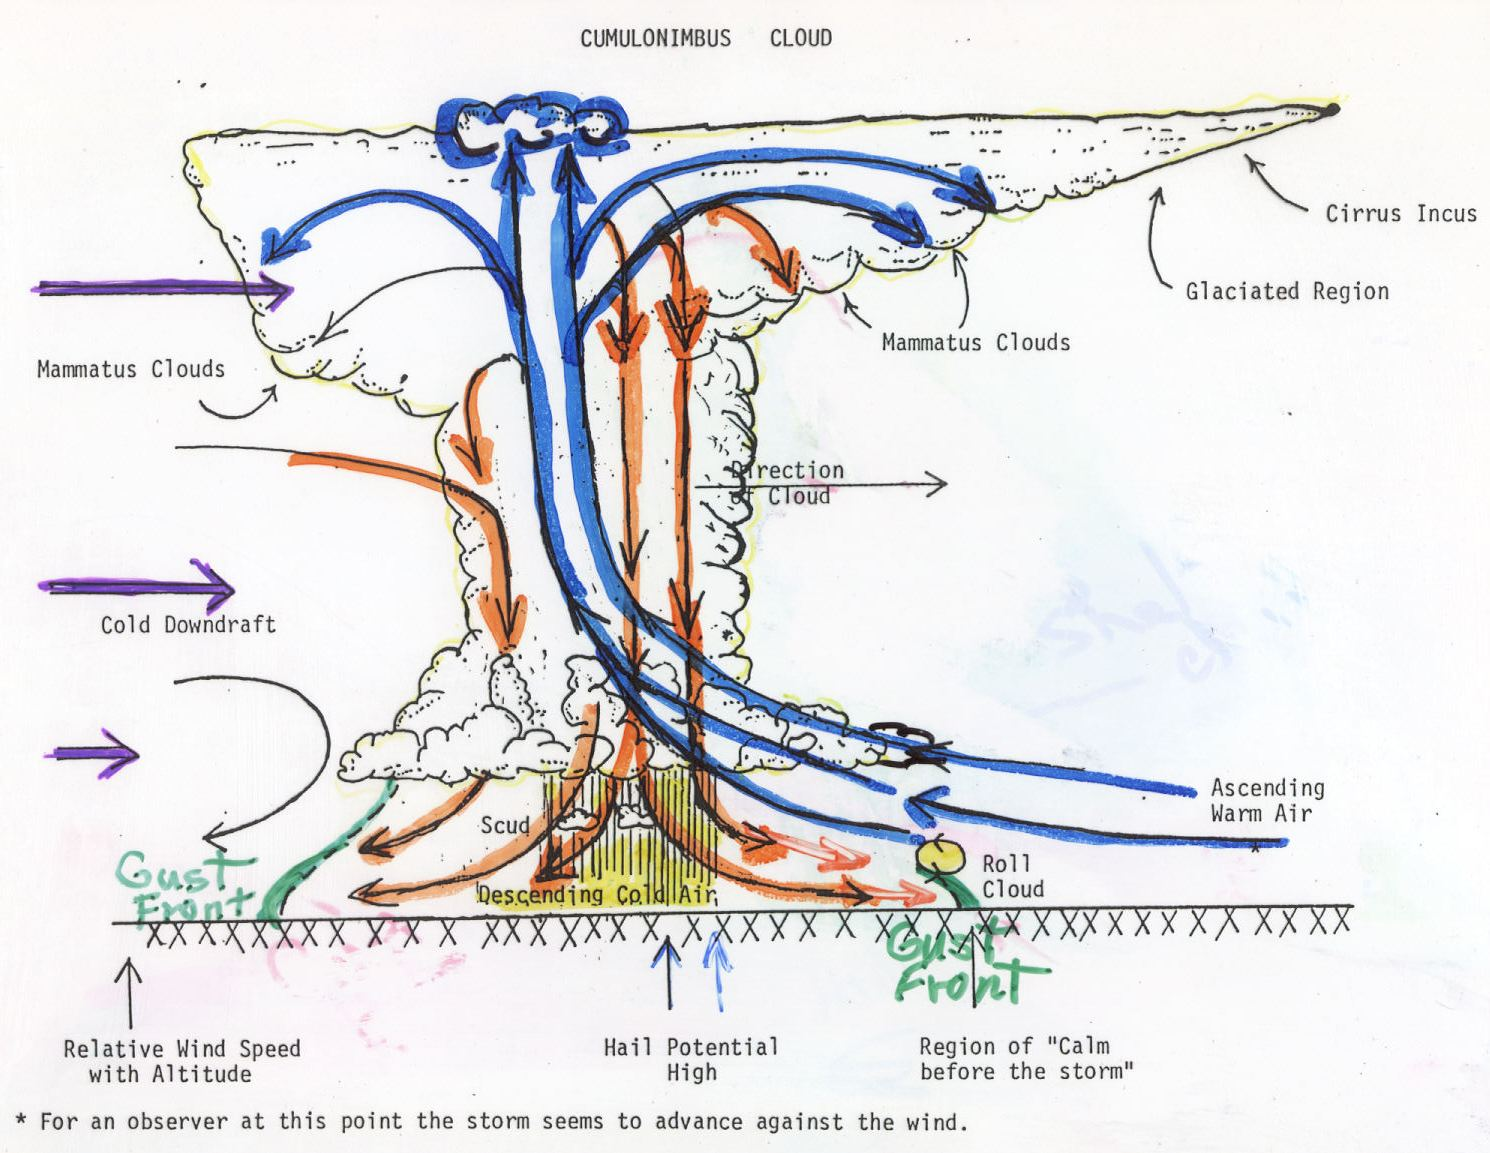
\includegraphics[width=\linewidth]{cloud}
    \caption{}
    \label{fig:cloud}
\end{figure*}
\begin{figure*}[t]
    \centering
    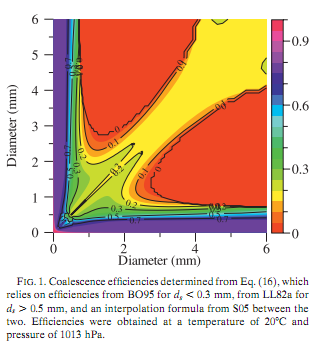
\includegraphics[width=0.75\linewidth]{coalesce_efficiency}
    \caption{}
    \label{fig:coalesce}
\end{figure*}
\begin{figure}[h]
    \centering
    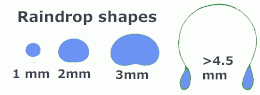
\includegraphics[width=0.75\linewidth]{raindrop_shapes}
    \caption{}
    \label{fig:raindrop}
\end{figure}
\begin{figure*}[t]
    \centering
    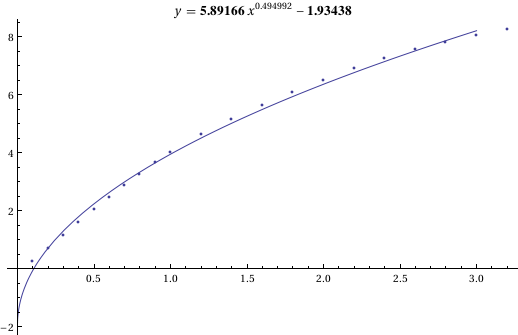
\includegraphics[width=0.75\linewidth]{terminal_velocity}
    \caption{}
    \label{fig:velocity}
\end{figure*}




Picture a huge room full of tiny droplets milling around. If one droplet bumps
into another droplet, the bigger droplet will "eat" the smaller droplet. This
new bigger droplet will bump into other smaller droplets and become even
bigger--this is called coalescence. Soon the droplet is so heavy that the cloud
(or the room) can no longer hold it up and it starts falling. As it falls it
eats up even more droplets. We can call the growing droplet a raindrop as soon
as it reaches the size of 0.5mm in diameter or bigger. If it gets any larger
than 4 millimeters, however, it will usually split into two separate drops.

The raindrop will continue falling until it reaches the ground. As it falls,
sometimes a gust of wind (updraft) will force the drop back up into the cloud
where it continues eating other droplets and getting bigger. When the drops
finally reach the ground, the biggest drops will be the ones that bumped into
and coalesced with the most droplets. The smaller drops are the ones that didn't
run into as many droplets. Raindrops are different sizes for two primary
reasons.


Dewpoint is the roof.


The more water vapor there is below the cloud, and the stronger the updrafts
that cause this water vapor to condense into cloud water or ice particles, the
more likely it is that precipitation will form within the cloud. 

So, a cloudy day with no precipitation indicates that there is either (1) not
enough water vapor available to the cloud for precipitation to form, or (2) that
the rising motion creating the cloud is not strong enough -- or both.     At the
opposite extreme is a tropical rain shower that has large amounts of water vapor
available to it (like the one pictured at the top of this page), and which can
rain heavily from even a small cloud with weak updrafts. 

In warm air masses, precipitation occurs primarily within localized shower
clouds that have strong updrafts. In cooler airmasses, precipitation (rain or
snow) usually occurs in large cloud systems associated with low pressure zones.
These low pressure zones usually form along the boundary between warm and cold
air masses, where the flow of air around the low pressure causes large areas of
weak rising motion as air from the warmer air mass flows up and over the colder
air mass.

Ref:

The development of the HiPE system:
design and experience report
http://user.it.uu.se/~kostis/Papers/hipe-sttt.pdf

Sensitivity of Cloud Droplet Growth to Collision and Coalescence Efficiencies in a
Parcel Model
http://journals.ametsoc.org/doi/pdf/10.1175/1520-0469(1998)055%3C2502%3ASOCDGT%3E2.0.CO%3B2

Hypothesis:

With lots of power, one could make the domain large enough for a meaningful simulation. Need TIME to traverse vapor area. Tried scaling down movement to simulate larger domain but it doesn’t increase the collisions  with large drops, just newly generated small ones.

\section{Model Limitations and Assumptions}

\section{Erlang}
Erlang is a high level functional language, originally developed by Eriksson in the 1990's to handle telecommunications workloads. It has since grown to enjoy wide-spread use in the telecommunications industry as the workhorse runtime in switches and interchanges. To this end, it has been designed from the ground up with a strong focus on concurrency, fault-tolerance, and, somewhat unlike its academic brethren, practicality.

From the perspective of the scientific programmer, working in FORTRAN or C, Erlang has very different and confusing semantics. In this section, I will try to address the more obvious quirks and argue my case for choosing Erlang as a potentially valuable tool in the scientific computing arena.

\subsection{Why not C?}
When we were all introduced to algebra at the beginning of our scientific careers, we learned that abstract representations of values such as $x$ were constant. Given two equations, $x = 3$ and $y = x$, we could say with confidence that $y = 3$ as well. This gave us very powerful tools for reasoning about complex systems of equations. We could directly substitute variables for their values, which might again be expressed in terms of variables. This is referred to as \emph{referential transparency}.

Unfortunately, when we all learned our first programming language, we were told that \emph{referential transparency} was no longer the way things worked. Suddenly, expressions like $X = X + 1$ were claimed to make sense and stranger still, this was considered a great and useful trick when writing programs. Imperative (read: sequential) languages like C and Java take this abandonment of mathematics to the extreme. It is virtually impossible to program these languages without making use of dynamically valued variables. As one might expect, by relaxing the notion that $x = x$ for any two instances of $x$ in the same context, referential transparency was lost and the ability to reason about the correctness of a program disappeared with it. We haven't even begun discussing the difficulty of reasoning about \emph{concurrent} algorithms written in this style. The good news is that many very talented people have put a heroic effort into writing programs in these languages which, almost by magic, produce mathematically accurate results. The bad news is that, typically, we are not those people. For you and I, the Programming Scientists, writing non-trivial programs in C which produce valid results is difficult and extremely time consuming. Personal experience and informal survey of my own colleagues suggests that upwards of 90\% of the time spent ``programming'' is actually spent searching for and correcting the inadvertent effects of changing the value of variables.

\subsection{Single Assignment Variables}
The irony, of course, is that we are specifically interested in \emph{mathematical} programming. Fortunately, there has been a minor revival of the functional programming movement lately. Highly specialized languages such as Mathematica provide a gentle reintroduction to mathematical programming for those who have forgotten their algebraic roots\footnote{Pun intended.}. These languages do suffer from their own problems, however. As demand for large-scale simulation increases with computing power, the need for parallel algorithms that can exploit multiple concurrent threads of execution become grows with it. Equally important is the ability of the programmer to successfully implement these algorithms.

\subsection{Pattern Matching}


\TODO 

\section{Implementation}




\end{document}


